\chapter{Optical Design}\label{app:optical_design}

\begin{appbox}
	Back to Section~\ref{subsect:thin_film:opto_elec:geom_cons}\hfill \hyperref[chapter:toc]{Main Table Of Content (TOC)}
\end{appbox}

Ideally, the most simple and naive design that can be envisioned is that coarsely presented in Figure~\ref{annfig:optics:outline}, Left: a supposedly ideal \gls{led}---hence the absence of excitation filter---shines its monochromatic light through a glass window onto a \gls{co2} sensitive luminescent thin film placed against the skin. The re-emitted light then reaches a photodiode covered by an emission filter to discard the parasitic diffused \gls{led} light that may otherwise reach it.

\begin{figure}
	\centering
	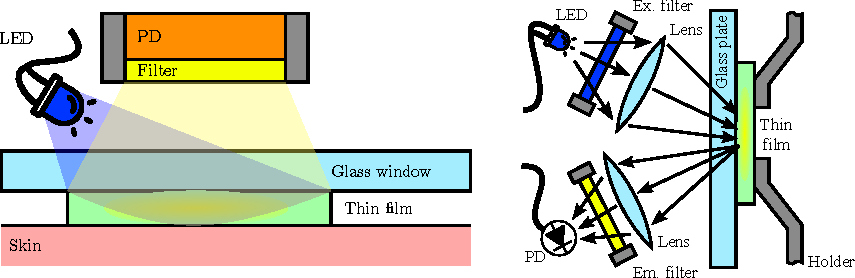
\includegraphics{2_appendices/optical_figures/naive_outline.pdf}
	\caption[Idealised and realistic optical setups.]{\textbf{Left:} crude outline of an idealised optical setup. \textbf{Right:} a more realistic version of the same optical setup.}
	\label{annfig:optics:outline}
\end{figure}

However, in the lab, the bulkiness of the emission filter, \gls{led} and photodiode mounts---in addition to the need for a second excitation filter---called for a larger optical setup made out of discrete optical components, since off the shelf filtered photodiodes were not available. The later setup is depicted in Figure~\ref{annfig:optics:outline}, Right, and can be seen as two distinct blocks:
\begin{itemize}
	\item[--] An illuminating block (Top), which purpose is to collect as much light as possible from the \gls{led} to form a spot of a given size $w$ on the thin film.
	\item[--] A collecting block (Bottom), which role is to maximise the amount of light 
	reaching the photodiode.
\end{itemize}

These two blocks will be placed as presented in Figure \ref{anfig:optics:meca_place}. At the bottom of the picture is the glass window (3~mm thick) while the two tilted blocks are the illuminating and collecting blocks, each one of them consisting of a mounting tube into which the different optical elements---\ie{} filters, lenses, \gls{led} and photodiode---will be housed. The diameter of the optical elements is 1~inch (25.4~mm), while the outer diameter of the optomechanics holding them is 30.5~mm. For practical reasons---\ie{} being able to mechanically integrate the two tubes into a larger assembly---two clearances were defined: one of 2~mm between the two optical blocks, and another one of 3~mm between the optical blocks and the glass window. These two clearances resulted in a 78.6{\degree} angle between the two blocks. Of note, each block is shown with a length of 10~mm for illustration purposes only, since their actual length is substantially greater in practice.

\begin{figure}
	\centering
	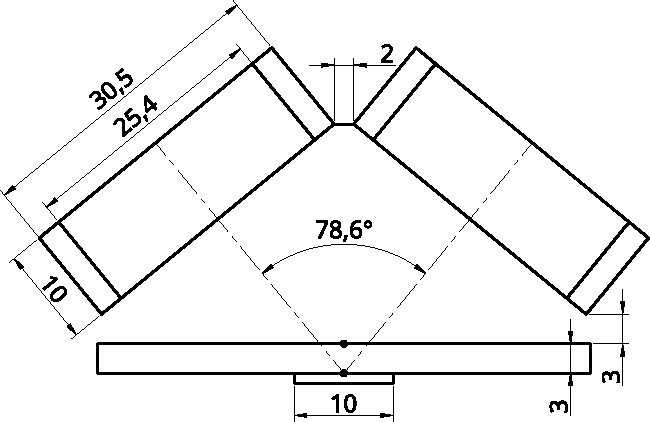
\includegraphics[scale=0.8]{2_appendices/optical_figures/meca_drawing.pdf}
	\caption[Placement of the different optical blocks.]{Placement of the different optical blocks. Bottom is the glass window, while the two tilted blocks are the illuminating and collecting blocks. See the text for a more complete description.}
	\label{anfig:optics:meca_place}
\end{figure}

It readily appears that the distance between the first optical element---\ie{} the lower end of the tubes---and the bottom of the glass window where the film will be placed is not constant. Neglecting the effect of diffraction in the glass window on the optical path length, and for an illuminated spot of 10~mm in diameter for instance, this distance is between 17 and 23~mm. In the remainder of the present study, this distant will be considered to be constant and equal to 20~mm, so that we can \enquote{unfold} the optical setup into two distinct and \emph{aligned} optical sub-assemblies---\ie{} wherein a given block sees the illumination spot perpendicular to its optical axis. Additionally, since the different lenses and other optical elements used are mounted by means of retaining rings (SM1RR, Thorlabs) the effective optical aperture of these sub-assemblies is equal to 0.9~inch (22.9~mm) instead of 1.0~inch (25.4~mm).

\section{Illumination block}

The scheme retained for the illuminating block is depicted in Figure \ref{anfig:optics:illuminating_th}. The \gls{led} is placed in front of a converging glass lens, which goal is to collect the light emitted by the \gls{led} and to concentrate it into a spot of the required dimension. For the sake of simplicity, the excitation filter was not considered, its optical properties and thickness being unknown---apart from its transmission, of course. This block must meet two targets: first, as much light as possible must be collected by the lens aperture, a condition which sets a maximum value for $d_{LL}$. Second, the rays emerging from the lens must converge onto the film and form a spot of diameter $w_S$, a condition which steer the choice of $d_{LL}$ and $d_{LS}$ values, as well as the lens focal length.

\begin{figure}
	\centering
	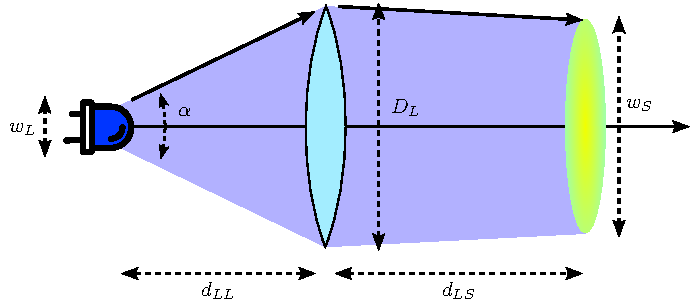
\includegraphics{2_appendices/optical_figures/illuminating_th_converted.pdf}
	\caption[Schematic drawing of the illuminating block.]{Schematic drawing of the illuminating block. The light is emitted by the \gls{led} of width $w_L$ with an maximum angle $\alpha$. $d_{LL}$ and $d_{LS}$ are the distances between the \gls{led} and the lens, and between the lens and the film, respectively. $D_L$ is the lens diameter, while $w_S$ is the width of the light spot, on the film.}
	\label{anfig:optics:illuminating_th}
\end{figure}

\subsection{Maximum \texorpdfstring{$d_{LL}$}{dLL}}\label{ansect:optics:maxdll}

The maximum $d_{LL}$ value is reached when the most diverging rays emerging from the \gls{led}---\ie{} those forming an angle $\alpha/2$ with the optical axis--- reach the border of the lens. This condition may be written
\begin{equation}
	\tan \left( \frac{\alpha}{2} \right) = \frac{D_L - w_L}{2 \cdot d_{LL}} \iff
	d_{LL} = \frac{D_L - w_L}{2 \cdot \tan \left( \frac{\alpha}{2}\right) }
\end{equation}

Taking Thorlabs' LED450L specifications---$\alpha/2=22\degree$, $w_L=4$~mm and $D_L=22.9$~mm---yields a maximum value $d_{LL,\mathrm{MAX}}$ of 23.4~mm. This means that if the \gls{led} is placed further away from the lens than 23.4~mm some rays will miss the lens and be lost, as can be seen in Figure \ref{anfig:optics:illuminating_lost_rays}, in red.

\begin{figure}
	\centering
	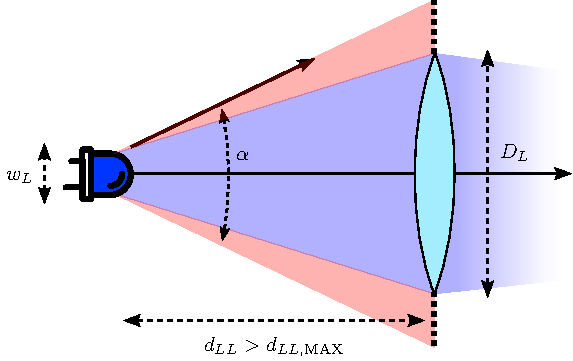
\includegraphics{2_appendices/optical_figures/illuminating_lost_rays_converted.pdf}
	\caption[$d_{LL}$ maximum value.]{If $d_{LL}$ is greater than the maximum value $d_{LL,\mathrm{MAX}}$ of 23.4~mm, some of the light emitted by the \gls{led} with an angle $\alpha$ will be lost (in red). This loss in turns reduces the amount of light concentrated onto the film (in blue).}
	\label{anfig:optics:illuminating_lost_rays}
\end{figure}

\subsection{Light Concentration onto the Film}

\subsubsection{Lens Focal Length}\label{ansubsect:optics:lens_f}

Since the light emerging from the \gls{led} is already collimated, all the rays emerging from it are comprised between the two most diverging rays at $\pm\alpha$/2. So as to form a spot of diameter $w_L < D_L$, the rays emerging from the lens must converge. The borderline case is depicted in Figure \ref{anfig:optics:illuminating_focal} and the corresponding equations are
\begin{equation}
	\tan \left( \frac{\alpha}{2} \right) = \frac{D_e}{2 \cdot f} \quad \text{with} \quad
	\frac{D_e}{2} = d_{LL}\cdot \tan \left( \frac{\alpha}{2} \right) + \frac{w_L}{2}
\end{equation}
\begin{equation}
	\text{hence}\quad f = d_{LL} + \frac{w_L}{2 \cdot \tan \left( \frac{\alpha}{2} \right)}
\end{equation}
wherein $f$ is the lens focal length. With the same numerical values as above, we find that the maximum $f$ value is equal to $d_{LL}+5.0$~mm. Taking the above-calculated $d_{LL}$ upper value of 23.4~mm for instance, this means that $f$ must be below 28.3~mm.

\begin{figure}
	\centering
	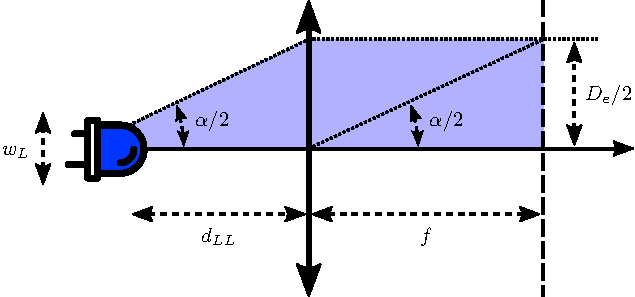
\includegraphics{2_appendices/optical_figures/illuminating_focal_converted.pdf}
	\caption[In the borderline case, the emerging rays are parallel to the optical axis.]{In the borderline case, the emerging rays are parallel to the optical axis. The diameter of the light spot projected onto the lens by the \gls{led} is noted $D_e$. The focal plane of the lens is represented with long dashes, while construction rays are represented using smaller dashes or dots.}
	\label{anfig:optics:illuminating_focal}
\end{figure}

\subsubsection{Adjusting the Spot Diameter}

If the two above conditions on the lens-to-\gls{led} distance $d_{LL}$ and focal length $f$ are met, as much light as possible is collected by the lens, and the rays emerging from it are converging. The relation between $d_{LS}$ and the size of the spot can then be expressed with the help of Figure \ref{anfig:optics:illuminating_spot} as
\begin{equation}
	\tan \left( \frac{\beta}{2} \right) = \frac{D_I - D_E}{2 \cdot f} = \frac{D_I - w_S}{2 \cdot d_{LS}}
\end{equation}
with
\begin{equation}
	D_I = 2 \cdot d_{LL} \cdot \tan \left( \frac{\alpha}{2} \right) + w_L\quad \text{and} \quad	D_E = 2 \cdot f \cdot \tan \left( \frac{\alpha}{2} \right)
\end{equation}
wherein $D_I$, $D_E$ and $\beta$ are defined in Figure \ref{anfig:optics:illuminating_spot}. These equations leads to:
\begin{equation}
	\begin{aligned}
		d_{LS} &= f \cdot \frac{D_I - w_S}{D_I - D_E}\\
		d_{LS} &= f \cdot  \frac{2\cdot d_{LL} \cdot \tan \left( \frac{\alpha}{2} \right) + w_L - w_S}{2\cdot \tan \left( \frac{\alpha}{2} \right) \cdot (d_{LL} - f) + w_L}
	\end{aligned}
\end{equation}

This latter equation is interesting because it tells us that if $f$ and $d_{LL}$ are chosen too close, a small inaccuracy on the \gls{led}-lens positioning---\ie{} $d_{LL}$---might result in an important $d_{LS}$ shift, and thus in an important change in the spot size $w_S$. Additionally, the practical considerations exposed while presenting Figure \ref{anfig:optics:meca_place} limits $d_{LS}$ to a minimum of approximately 20.2~mm.

\begin{figure}
	\centering
	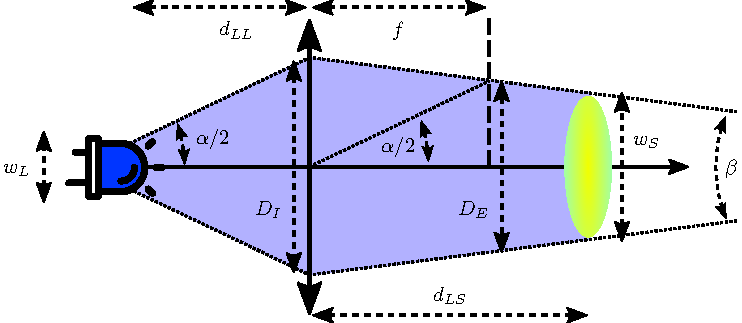
\includegraphics{2_appendices/optical_figures/illuminating_spot_converted.pdf}
	\caption[Complete annotated schematic of the illuminating block.]{Complete annotated schematic of the illuminating block. $D_I$ is the diameter of the light spot produced by the \gls{led} onto the lens surface, and $D_E$ is the diameter of the emerging light beam in the focal plane. $\beta$ is the angle of the converging rays emerging from the lens.}
	\label{anfig:optics:illuminating_spot}
\end{figure}

\subsubsection{Practical Realisation}

To sum up the above considerations, we must meet the following conditions (using a 16~mm focal length lens, as detailed below):
\begin{enumerate}[label=\textit{(\roman*)}]
	\item $d_{LL} > 19$~mm because of the presence of the excitation filter of thickness 6.3~mm, plus 8.7~mm of lens thickness (16~mm focal minus 7.3 back focal length), 2~mm of retaining ring, 1.7~mm of \gls{led} bulb, rounded to the upper value to allow for positioning error and in order to avoid crushing the \gls{led} into the filter.
	\item $d_{LL} < 23.4$~mm not to lose any \gls{led}-emerging rays, as explained in Section \ref{ansect:optics:maxdll}.
	\item $f < d_{LL} + 5.0~mm$ to allow for converging rays emerging the lens, as explained in the previous section.
	\item $d_{LS} > 23.8~mm$ due to the practical consideration exposed in Figure \ref{anfig:optics:meca_place}.
\end{enumerate}

In practice, if $d_{LL}$ and $d_{LS}$ can be changed continuously, there is only a limited number of focal lengths available from the manufacturer. For instance, Thorlabs' standards focal lengths are 25.4~mm or 16.0~mm for 1" lenses. Since the optical system should remain compact for practical reasons, Thorlabs' $f=16$~mm condensing lens (ACL25416U) was finally chosen. In this configuration, the shortest possible $d_{LL}$ of 19~mm and a spot of diameter $w_S=10$~mm lead to a $d_{LS}$ distance of 23.3~mm. However, the latter being slightly below the 23.8~mm of constraint \textit{(iv)}, it was rounded up to 24~mm, which would result in practice to a spot slightly smaller than 10~mm in diameter (9.7~mm). For reference, Figure \ref{anfig:optics:lens_spot_distance} represent $d_{LS}$ as a function of $d_{LL}$ for a variety of spot diameters $w_S$. Finally, Figure \ref{anfig:optics:illuminating_meca}, presents both a schematic mechanical drawing reporting the above dimensions and a 3D-view of the resulting opto-mechanical assembly.

\begin{figure}
	\centering
	\includegraphics{2_appendices/optical_figures/tikz/out/lens_spot_distance.pdf}
	\caption[Distance between the lens and the thin film as a function of the \gls{led}-lens distance for various spot sizes.]{Distance between the lens and the thin film as a function of the \gls{led}-lens distance for various spot sizes. Calculations were made with a 16~mm focal length lens. The green square indicates constraints \textit{(i)} and \textit{(iv)}.}
	\label{anfig:optics:lens_spot_distance}
\end{figure}

\begin{figure}[h!]
	\centering
	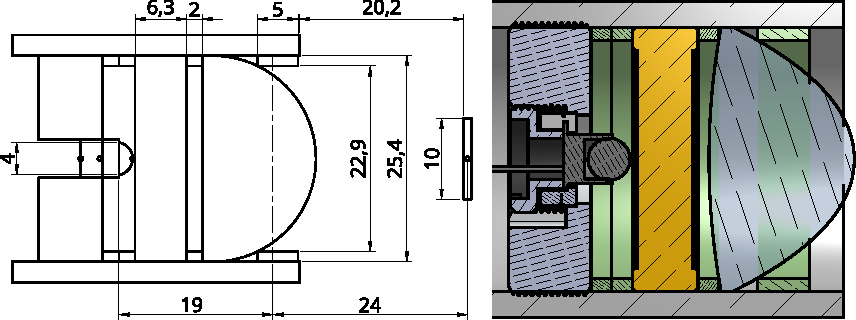
\includegraphics{2_appendices/optical_figures/illuminating_meca}
	\caption[Mechanical drawing (Left) and 3D section-view (right) of the final illuminating block assembly.]{Mechanical drawing (Left) and 3D section-view (right) of the final illuminating block assembly. From left to right (all parts are Thorlabs'): an \gls{led} mount (S1LEDM) holding the \gls{led} (LED450L), two retaining ring (SM1RR), the excitation shortpass filter (FES450), a third retaining ring (SM1RR), the lens (ACL25416U), and a large retaining ring (SM1RRC). All elements are mounted into a SM1 threaded tube. The rectangle element on the right part of the mechanical drawing depicts the thin film. Note that the focal plane of the lens is plotted as a dashed line.}
	\label{anfig:optics:illuminating_meca}
\end{figure}

\section{Light Collection block}

The scheme retained for the collecting block is depicted in Figure \ref{anfig:optics:collecting_th}. The light collection block aims at collecting as much light as possible from the fluorescent film, but contrary to the \gls{led}, the film emits light in all directions---\ie{} it is an isotropic source. Thus, it would seem intuitive to place the first collecting lens as close as possible to the film. However, since the focal of the lens cannot be arbitrarily small, placing it too close from the film would result in rays emerging from the lens diverging from the optical axis, and therefore not collectible by the photodiode. In addition, the mechanical considerations presented in Figure \ref{anfig:optics:meca_place} prevents the first lens to be placed closer than 20.2~mm from the film. Please note that the illuminated spot also emits light opposite to the photodiode, so 50\% of the light re-emitted by the film is lost anyway. Unless a mirror, or some kind of reflective or highly diffusive---\ie{} white---coating is placed below the film, for instance. This possibility is not further explored in the present study however.

\begin{figure}
	\centering
	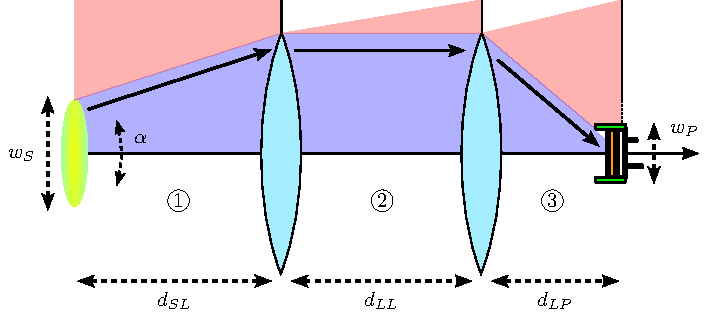
\includegraphics{2_appendices/optical_figures/collecting_th_converted.pdf}
	\caption[Principle schematic of the collecting block.]{Principle schematic of the collecting block. The light is emitted by the film spot of width $w_S$ illuminated by the \gls{led}. $d_{SL}$, $d_{LL}$ and $d_{LP}$ are the distances between the spot and the first lens, between the two lenses, and between the second lens and the photodiode, respectively. $w_P$ is the width of the photodiode. In mauve are the rays contributing to the signal measured at the photodiode, while in pink are the rays that are lost. The light-collecting surface of the photodiode is coloured in orange, while its mechanical enclosure is green.}
	\label{anfig:optics:collecting_th}
\end{figure}

As can be seen in Figure \ref{anfig:optics:collecting_th}, the path of a light ray can be decomposed into three travels, delimited by the two deviations caused by the lenses: \Circled{1} between the film and the first lens, \Circled{2} between the two lenses, and \Circled{3} between the second lens and the photodiode. While the amount of light reaching the first lens relative to the total amount of light emitted by the spot can be easily expressed analytically (see Section \ref{ansect:optics:accuracy}), the calculation quickly becomes unfeasible in a more general case involving several lenses and other opto-mechanical components. Thus, it was decided to create a basic ray-tracing engine\footnote{This approach was quite artisanal, and I would advise readers to use dedicated software---such as Zemax or the like---if they need to perform similar work. However, building a simple ray-tracing engine for this specific use case was a relatively quick process---\ie{} taking only a few days of work---and may still be faster than learning to navigate Zemax, which can be somewhat labyrinthine.} that would launch rays uniformly from the spot, and measure the number of rays reaching the photodiode in the end. Then, the three parameters $d_{SL}$, $d_{LL}$ and $d_{LP}$ were optimised so as to maximise the amount of light collected at the photodiode. As in the previous section, light propagation through the emission filter was not considered, and the latter filter was only considered in terms of its physical dimensions.

\subsection{Ray-Tracing}

The main advantage of ray tracing is that it is quite simple to mathematically express the conditions that a ray must satisfy in order to reach the photodiode. These conditions are the following:
\begin{enumerate}[label=\textit{(\roman*)}]
	\item A ray emitted by the spot must reach the surface of the first lens.
	\item A ray emerging from the first lens must reach the surface of the second lens.
	\item A ray emerging from the second lens must reach the photodiode's surface without being blocked by its mechanical enclosure.
\end{enumerate}

The spot is uniformly divided into a number $n_{pts}$ of points, and each spot point uniformly launches a number $n_{rays}$ of rays. These three conditions are then checked sequentially for a given ray, if the condition tested is false, the considered ray is terminated and another ray is launched, if the condition is true, the ray continues its travel until the next condition. If the three conditions are met, the ray is considered as \enquote{detected}. These conditions are depicted in Figure \ref{anfig:optics:collecting_cond}. The following paragraphs detail the different steps leading to the detection of a ray by the photodiode.

\begin{figure}
	\centering
	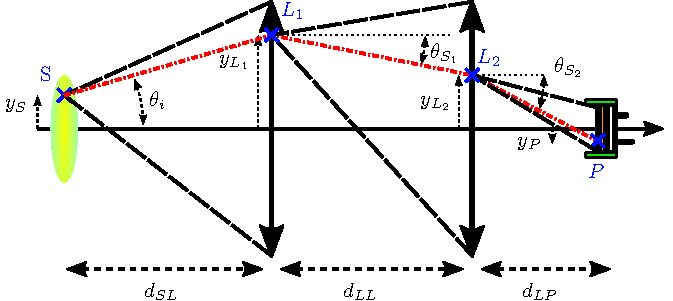
\includegraphics{2_appendices/optical_figures/collecting_cond_converted.pdf}
	\caption[Study of a ray emerging with an initial angle $\theta_i$ from a source point $S$.]{Study of a ray emerging with an initial angle $\theta_i$ from a source point $S$ (ordinate $y_S$). Its path is represented with a red dashed-doted line. It emerges successively from the two lenses at points $L_1$ and $L_2$ with the angles $\theta_{S_1}$ and $\theta_{S_2}$. The conditions \textit{(i)--(iii)} are represented with the long-dashed black lines. The red ray is valid / detected because it is always between these two lines.}
	\label{anfig:optics:collecting_cond}
\end{figure}

\subsubsection{Reaching the First Lens}

Considering a source point $S$ of ordinate $y_S$, and a light ray emitted by $S$ at an angle $\theta_i$ with respect to the optical axis. Reaching the second lens means that $y_{L_1}$, the ordinate of the intersection of this ray and the first lens plane must satisfy
\begin{equation}\label{aneq:optics:cond_1}
	-D_L < 2\cdot y_{L_1} < D_L \quad \text{wherein} \quad	y_{L_1} =  d_{SL} \cdot \tan(\theta_i) + y_S
\end{equation}

If the condition described by equation \ref{aneq:optics:cond_1} is satisfied, the ray travels further---\ie{} it will exit the lens---otherwise it is terminated.

\subsubsection{Deviation by the Lenses}

Once the ray reached the first lens in $L_1$, its emerging angle $\theta_{S_1}$ can be computed, which value will determine whether the ray reaches the second lens or not. Considering Figure \ref{anfig:optics:collecting_lens_int}, we have
\begin{equation}\label{aneq:optics:dev1}
	f\cdot \tan(\theta_{S_1}) = f\cdot \tan(\theta_i) - y_{L_1}\quad \text{which leads to} \quad \theta_{S_1} = \arctan \left( \frac{f\cdot \tan(\theta_i) - y_{L_1}}{f} \right)
\end{equation}

\begin{figure}
	\centering
	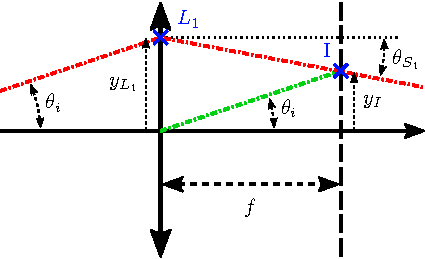
\includegraphics{2_appendices/optical_figures/collecting_lens_int_converted.pdf}
	\caption[Deviation of an incident ray by a converging lens of focal $f$.]{Deviation of an incident ray by a converging lens of focal $f$. The green ray is parallel to the incident red ray coming from the left of the picture with an angle $\theta_i$. The focal plane of the lens is represented by a long-dashed line. The point $I$ is the intersection between the real emerging ray in red, the fictitious green ray and the focal plane.}
	\label{anfig:optics:collecting_lens_int}
\end{figure}

It is clear that the same train of thought can be applied to the second lens, substituting $\theta_{S_1}$ to $\theta_i$, $\theta_{S_2}$ to $\theta_{S_1}$ and $L_2$ to $L_1$, we have
\begin{equation}
	f \cdot \tan( \theta_{S_2}) = f\cdot \tan(\theta_{S_1}) - y_{L_2} \quad \text{leading to} \quad \theta_{S_2} = arctan \left( \frac{f\cdot tan(\theta_{S_1}) - y_{L_2}}{f} \right)
\end{equation}

\subsubsection{Reaching the Second Lens}

As for the first lens, we can write the condition for the ray emerging from the surface of the first lens to reach the second one as
\begin{equation}\label{aneq:optics:cond_2}
	-D_L < 2\cdot y_{L_2} < D_L \quad \text{wherein}\quad y_{L_2} =  d_{LL} \cdot \tan(\theta_{S_1}) + y_{L_1}
\end{equation}

Using equation \ref{aneq:optics:dev1} leads to
\begin{equation}
	y_{L_2} =  d_{LL} \cdot \tan(\theta_i) + y_{L_1} \cdot \left( \frac{f - d_{LL}}{f} \right)
\end{equation}

As before, if the condition described by equation \ref{aneq:optics:cond_2} is true, it means that the ray reaches the second lens and can travel further. Otherwise, it is terminated.

\subsubsection{Reaching the Photodiode}

To reach the photodiode, a ray emerging from the second lens must fulfil two criteria: \textit{(i)} it must be directed towards the surface of the photodiode and \textit{(ii)} it must not be blocked by the mechanical enclosure of the photodiode. These two conditions are illustrated in Figure \ref{anfig:optics:collecting_pd_cond}.

\begin{figure}
	\centering
	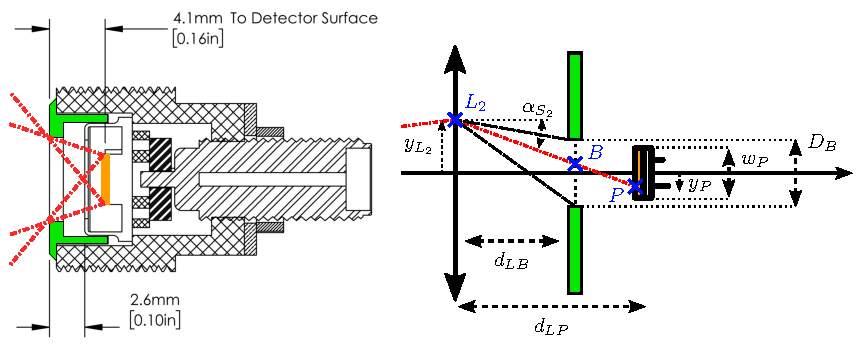
\includegraphics{2_appendices/optical_figures/pd_aperture_converted.pdf}
	\caption[Drawing and schematic view of the mounted photodiode.]{\textbf{Left:} drawing of the mounted photodiode with the light-sensitive surface in orange and the potentially blocking elements in green. In red, some borderline rays are plotted: rays cannot reach the surface of the photodiode if they are more diverging than the plotted ones. \textbf{Right:} schematic view of the photodiode when placed in front of the second lens. The aperture $D_B$ of the blocking element (in green), limits the collection of rays too diverging compared to the optical axis. This aperture is placed at a distance $d_{LB}$ from the lens. $B$ is the point located at the intersection between the ray and the blocker plane.}
	\label{anfig:optics:collecting_pd_cond}
\end{figure}

The blocking part of the photodiode can be considered as a infinitely thin plane with one circular aperture of diameter $D_B$ located at a distance $d_{LP}$ of the second lens. In such a case, the condition for a ray to pass through this aperture is
\begin{equation}
	-D_B < 2 \cdot y_B < D_B \quad \text{with} \quad y_B = d_{LB} \cdot \tan( \theta_{S_2} ) + y_{L_2}
\end{equation}
and that for a ray to reach the light-sensitive surface of the photodiode is
\begin{equation}
	-w_P < 2 \cdot y_P < w_P \quad \text{with} \quad y_P = d_{LP} \cdot \tan( \theta_{S_2} ) + y_{L_2}
\end{equation}

\subsection{Accuracy Considerations}\label{ansect:optics:accuracy}

Now that the conditions for a given light ray emitted by the luminescent spot to reach the photodiode are known. The next step is to study the accuracy of the designed ray tracing engine in terms of number of rays launched \textit{versus} prediction error. Indeed, when using a ray-tracing algorithm, one must ensure that \emph{enough} rays are being launched, and there is always a trade-off between the reached accuracy---which increases with an increasing number of rays---and performance---with a simulation time also increasing with the number of rays. The total number of rays launched can be expressed as
\begin{equation}
	N_\mathrm{rays} = n_\mathrm{pts} \cdot n_\mathrm{rays}
\end{equation}
wherein $n_\mathrm{pts}$ is the number of points into which the light source is divided, and $n_\mathrm{rays}$ is the number of rays emitted by each one of these source points. To ascertain the accuracy of the devised ray-tracing engine, it was tested on the first condition that was mentioned in the collecting block analysis, which can be translated into the following question: which amount of emitted light by the spot does reach the surface of the first lens? The latter can be expressed exactly as
\begin{equation}
	E_L = \frac{1}{2\cdot \pi \cdot w_S} \cdot \int_{-\frac{w_S}{2}}^{+\frac{w_S}{2}} \arctan \left( \frac{D_L / 2 - y}{d_{SL}} \right) - \arctan \left( \frac{-D_L / 2 - y}{d_{SL}} \right) dy
\end{equation}
wherein $E_L$ is the relative energy reaching the surface of the first lens, compared to the total energy re-emitted by the spot. $E_L$ thus has a theoretical maximum value of 50\%, which is reached when the lens is placed against the spot ($d_{SL}$=0), and its overall outline is represented in Figure \ref{anfig:optics:exact_pc_dist}. As can be seen, $E_L$ decreases sharply with an increase in $d_{SL}$. For instance, the amount of light that can be collected by a 1~inch lens (effective diameter of $D_L$=22.9~mm) from an isotropic 1~cm circular spot drops from 26.6\% at 10~mm down to 16.4\% at 20~mm and 11.5\% at 30~mm. Since $E_L$ can be exactly known in this way, its theoretical value can be compared with the ray-tracing results to ascertain the accuracy of the devised ray-tracing engine in a simple case.

\begin{figure}
	\centering
	\includegraphics{2_appendices/optical_figures/tikz/out/aperture_first_lens.pdf}
	\caption[Relative power $E_L$ collected at the surface of the lens, as a function of the object / lens distance $d_{SL}$.]{Relative power $E_L$ collected at the surface of the lens, as a function of the object / lens distance $d_{SL}$. $E_L$ quickly drops from its theoretical maximum of 50\% at $d_{SL}$=50~mm down to below 10\% for a $d_{SL}$ above 35~mm.}
	\label{anfig:optics:exact_pc_dist}
\end{figure}

The influence of $n_\mathrm{pts}$ and $n_\mathrm{rays}$ were investigated separately, as can be seen in Figure \ref{anfig:optics:nn_influence}. Taking into account the scale difference between the two graphs, it appears that $n_\mathrm{rays}$ has a greater influence than $n_\mathrm{pts}$ on the accuracy. Indeed increasing $n_\mathrm{pts}$ above 300 source points has no further effect on the resulting accuracy, while higher $n_\mathrm{rays}$ values continue to improve it. The influence of both parameters can be seen in Figure \ref{anfig:optics:nn_influence_3d}. For all three figures, $d_{SL}$=20~mm, $w_S$=10~mm, $D_L$=25.4~mm.

\begin{figure}
	\centering
	\includegraphics{2_appendices/optical_figures/tikz/out/acc_influence.pdf}
	\caption[Amount of light collected as a function of the number of source points and rays.]{\textbf{Left:} amount of light collected as a function of the number of source points used ($n_\mathrm{rays}$=5000). \textbf{Right:} amount of light collected as a function of the number of rays per source point used ($n_\mathrm{pts}$=5000). In both cases the ground truth corresponds to the exact calculus.}
	\label{anfig:optics:nn_influence}
\end{figure}

\begin{figure}
	\centering
	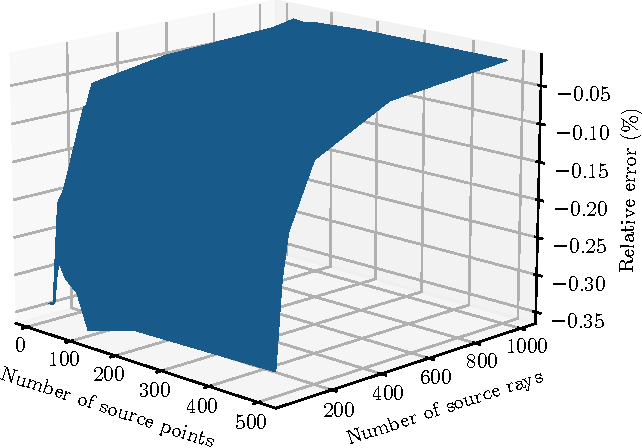
\includegraphics{2_appendices/optical_figures/nn_influence_3d.pdf}
	\caption{3D plot of the influence of both $n_\mathrm{pts}$ and $n_\mathrm{rays}$ on the relative error on $E_L$.}
	\label{anfig:optics:nn_influence_3d}
\end{figure}

It can be concluded that an $n_\mathrm{pts}$ value above 200 is enough, while an $n_{rays}$ of 500 is a good starting value, leading to a relative error of 0.2\% and a computation time of 0.15~s. It must be stressed out that this choice is of course essentially arbitrary, and that higher figures could always be chosen, yielding even lower error values. However, given the approximations that were used---\eg{} no influence of the filters, no backscattered rays or internal reflections inside the lenses, \etc{}---the overall model accuracy is likely to be driven by the latter rather than by ray-tracing Monte-Carlo-like errors. To give an idea of the orders of magnitude involved, the underlying Python code was optimised so that up to $10^6$ rays can be traced in $\sim$1.3~s, and the simulation time is proportional to the number of rays traced.

\FloatBarrier

\subsection{Positioning the Optical Elements}

With the help of the above-described ray tracing engine, an approximation of the relative amount of light collected at the photodiode $E_P$ can be computed as a function of $d_{SL}$, $d_{LL}$ and $d_{LP}$. The maximum value of $E_P$ as well as the corresponding $d_{SL}$, $d_{LL}$ and $d_{LP}$ values can thus be found using a standard optimisation algorithm. As an illustration, and since representing $E_P$ as a function of its three parameters is unfeasible, the influence of $d_{LL}$ on $E_P$ for several $d_{SL}$ and $d_{LP}$ values was plotted in Figure \ref{anfig:optics:d_ll_influence}. Similar graphs can of course be obtained for $d_{SL}$ and $d_{LP}$.

\begin{figure}
	\centering
	\includegraphics{2_appendices/optical_figures/tikz/out/dll_influence.pdf}
	\caption{Influence of $d_{LL}$ on $E_P$ for several $d_{SL}$ and $d_{LP}$ values.}
	\label{anfig:optics:d_ll_influence}
\end{figure}

\subsubsection{Setting Boundaries}

To maximise the amount of light collected at the photodiode, the following optimisation problem must be addressed, \ie{} the $(d_{SL}, d_{LL},d_{LP})$ values which fulfil the following relation must be found:
\begin{equation}
	\left( d_{SL}, d_{LL},d_{LP} \right) = \smashoperator{\argmax_{d_{SL},d_{LL},d_{LP}}}(E_P)\quad \text{wherein} \quad \begin{cases}
		d_{SL} \in B_{SL}\\
		d_{LL} \in B_{LL}\\
		d_{LP} \in B_{LP}
	\end{cases}
\end{equation}
with $B_{SL}$, $B_{LL}$ and $B_{LP}$ delimiting the boundaries for the three $d_{XX}$ variables. At first, as earlier presented in Figure \ref{anfig:optics:meca_place}, $d_{SL}$ should be at least 20.2~mm. Alas, due to the thicknesses of the mounting ring and lens, this distance must me extended up to 30.8~mm. Then, due to the size of the lenses, $d_{LL}$ should be at least 14.0~mm, but since the low-pass filter must also be added to the assembly, this distance is raised up to 21.4~mm. $d_{LP}$, on its part, is at least 9.4~mm. No upper values do exist in theory. However, to speed up the optimisation process, we set an upper bound of 50~mm for the three $d_{XX}$ variables. To sum up (all lengths in mm):
\begin{equation}
	\begin{cases}
		d_{SL} \in B_{SL}=[30.8;50.0]\\
		d_{LL} \in B_{LL}=[21.4;50.0]\\
		d_{LP} \in B_{LP}=[9.4;50.0]
	\end{cases}
\end{equation}

% d_SL: 20.2 + 1.9 + 8.7 = 30.8
% d_LL: 14mm (lens thickness) + 7.43 (filter + part of mounting ring) = 21.4mm
% d_LP: 9.4 mm = 5.3 (lens back) + 4.1 (PD front)

\subsubsection{Optimisation Results}

The above-given limits and optimisation problem were fed to a numerical solver---namely the \verb|differential_evolution| program from the SciPy Python library\cite{scipy2020}, itself based on an algorithm proposed by Storn \etal{}\cite{storn1997}. The algorithm converged towards the following optimal distances to maximise $E_L$:
\begin{equation}
	\begin{cases}
		d_{SL}=30.8\text{~mm}\\
		d_{LL}=21.5\text{~mm}\\
		d_{LP}=11.2\text{~mm}
	\end{cases}
\end{equation}
which yield an $E_P$ value at the photodiode of 5.9\%. This value can be compared with the maximum value of $E_L$=11.3\% received by the surface of the first lens for $d_{SL}$=30.8~mm. One may also note that $d_{SL}$ and $d_{LL}$ are equal---or extremely close---to their lower bounds.

Out of curiosity, we performed the same optimisation with no lower bounds for $d_{SL}$ and without taking the filter into account---\ie{} setting the lowest $d_{SL}$ value to 10.6~mm and the lowest $d_{LL}$ value to 14~mm. In such a configuration, we found a maximum amount of light collected of 6.8\%, a value which is reached for $d_{SL}$=30.6~mm, $d_{LL}$=14.0~mm and $d_{LP}$=9.4~mm ($E_L$=11.3\% at $d_{SL}$=30.6~mm)

It is also interesting to note that to reach such levels---in the 10\% region---in a \emph{proximity} configuration---that is to say with the photodiode located directly in front of the spot---a spot / photodiode distance $d_{SP}$ below 8.6~mm would be necessary. This result is not significantly modified by the size of the spot, with a $d_{SP}$ below 9.4~mm still required even with a spot size of only 3~mm. The calculations leading to this result are essentially the same as those presented in section \ref{ansect:optics:accuracy}.

\subsubsection{Practical Realisation}

As was the case for the illuminating block, the above presented light collection scheme must be implemented in the real world, preferably using off-the-shelf optical components. The whole assembly fits into a 2~inches long tube, as can be seen in Figure \ref{anfig:optics:collecting_assembly}, and can be build using standard Thorlabs components.

% 2.4mm : measured gap when the lens is against the filter + 0.1
% 4.4mm gap at 9.4mm -> **6.2mm** gap at 11.2mm

\begin{figure}
	\centering
	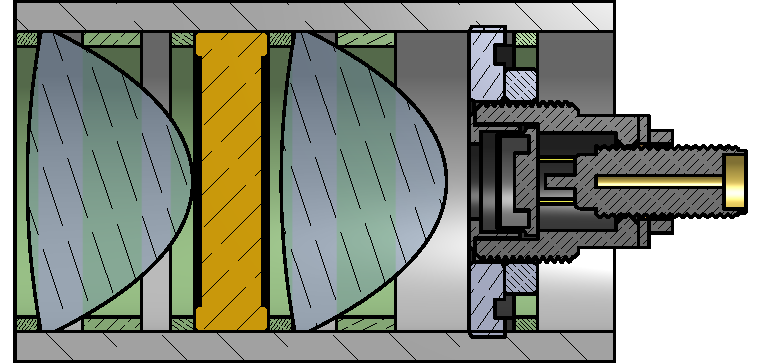
\includegraphics{2_appendices/optical_figures/collecting_assembly.pdf}
	\caption[Cut view of the whole collecting block assembly.]{Cut view of the whole collecting block assembly (all part numbers are Thorlabs'). In green are the thin (SM1RR) and thick (SM1RRC) retaining rings, in transparent blue are the two lenses (ACL25416U), and in yellow is the filter (FEL0450). Finally the block on the right is composed of the photodiode (SM05PD1A) mounted into a SM1 to SM05 thread adapter (SM1A6) and locked with a SM05 ring (SM05NT).}
	\label{anfig:optics:collecting_assembly}
\end{figure}

\section{Complete Assembly}

A \gls{pla} 3D-printed contraption was designed to hold the illumination and collection blocks altogether, and point them at the fluorescent thin film placed behind the glass window, as can be seen in Figure \ref{fig:thin_film:opto_elec:optics_cut} of the main text.

\section{Link Budget}\label{ansect:optics:link_budget}

To appropriately size the \gls{led}'s power and photodiode transimpedance amplifier's gain, a link budget was calculated, considering the optical setup as a whole. Of note, the values given below are mainly use as orders of magnitude and should \textbf{not} be taken too literally.

Starting with the \gls{led}, an optical power of 10~mW was taken, slightly above the 7~mA of nominal \gls{dc} power from the LED450L (Thorlab), but below its maximal one ($\sim$20~mW)
\begin{equation}
	P_\mathrm{LED, opt} = 10~\mathrm{mW}
\end{equation}

The illuminating assembly was designed so that all the light emitted by the \gls{led} reaches the film. The film absorbance and conversion factor $T_{film}$ is then function of the film absorbance $A$ and quantum yield $\Phi$. A value of 0.1 was deemed reasonable since the absorbance can be tuned by either changing the film thickness, dye concentration, or both, and since the quantum yields of the dyes---\ie{} \gls{hpts} and \gls{rudpp} is relatively high
\begin{equation}
	T_\mathrm{film} = A \cdot \Phi = 0.1
\end{equation}

The collecting assembly is then able to collect 5.9\% of the light re-emitted by the film, as mentioned above.
\begin{equation}
	T_\mathrm{collect} = 0.059
\end{equation}

The optical power received at the photodiode is thus
\begin{equation}
	P_\mathrm{PD,opt} = P_\mathrm{LED,opt} \cdot T_\mathrm{film} \cdot T_\mathrm{collect} \approx 50~{\mu}W
\end{equation}

Ideally generating a photocurrent given by
\begin{equation}
	\begin{aligned}
		E_\mathrm{photon} &= h \cdot \nu = \frac{h \cdot c}{\lambda} \\
		\frac{dn_\mathrm{photons}}{dt} &= \frac{P_\mathrm{PD,opt}}{E_\mathrm{photon}} = \frac{P_\mathrm{PD,opt} \cdot \lambda}{h \cdot c} \\
		dQ &= dn_\mathrm{photons} \cdot e \cdot \eta_\mathrm{PD}
	\end{aligned}
\end{equation}
wherein e=$1.60\times10^{-19}$~C is the elementary charge, h=$6.63\times10^{-34}$~J.s Plank's constant, c=$3.00\times10^{8}$~m.s$^{-1}$ light's celerity, $\lambda$=450~nm, and $\eta_\mathrm{PD}$ the quantum yield of the photodiode, taken equal to 0.1. Finally, the photocurrent produced by the photodiode may thus be written:
\begin{equation}
	\begin{aligned}
		I_\mathrm{PD} &= \frac{dQ}{dt} = \frac{P_\mathrm{PD,opt} \cdot \lambda \cdot e \cdot \eta_\mathrm{PD}}{h \cdot c} \\
		I_\mathrm{PD} &\approx 1.7~\mu A
	\end{aligned}
\end{equation}

To reach an output voltage in the range of 100-500~mV, a trans-impedance gain of 10$^5$~V.A$^{-1}$ is thus needed. The selected first-stage amplifier AMP102 (Thorlabs) can reach 10$^5$~V.A$^{-1}$ and a second stage of amplification could be used if the signal is still too low. I did not expect the latter situation to happen, though, since some factors taken to establish this link budget were rather pessimistic---$T_\mathrm{film}$, in particular.

\begin{appbox}
	Back to Section~\ref{subsect:thin_film:opto_elec:geom_cons}\hfill \hyperref[chapter:toc]{Main Table Of Content (TOC)}
\end{appbox}